\documentclass[tikz]{standalone}

\usetikzlibrary {folding}
\tikzset{
  scale text width/.style 2 args={
    text width={(#2-2*(\pgfkeysvalueof{/pgf/inner xsep}))/(#1)},
    scale={#1}}}

\begin{document}
\begin{tikzpicture}[scale=10]
  \pic [
    folding line length=6mm,
    transform shape,
    inner sep=+.15em,
    face 1= {
      \node[scale text width={.2}{6mm}] {
        \textbf{Cayendo en las redes de Venecia}\\[1.3em]JJ Merelo
      };
    },
    face 2= { \node{ Tibi }; },
    face 3= { \node{\tiny Marce}; },
    face 4= { \node{\tiny Evangelista}; },
    face 5= { \node[anchor=center] {
\includegraphics[width=0.6cm]{img/noqrbig} }; },
    face 6= { \node[anchor=center] {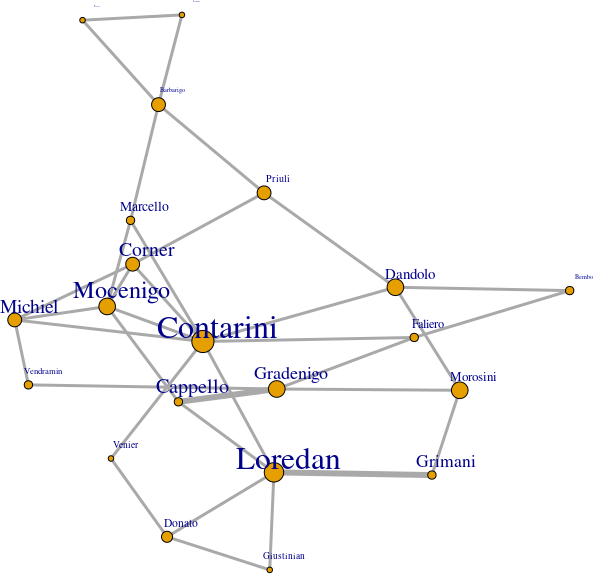
\includegraphics[width=0.6cm]{img/dogos} };}
  ]
  { cube folding };
\end{tikzpicture}

\end{document}